\documentclass[a4paper,10pt]{article}
\usepackage{natbib}
\usepackage{amsmath,amssymb}
\usepackage{graphicx}
\usepackage{fancyvrb}
\usepackage{booktabs}
\usepackage{tikz}
\usepackage{threeparttable}
% \usetikzlibrary{positioning,shapes,shadows,arrows,fit,backgrounds,decorations.pathmorphing}

\title{Newton--Raphson for \citet{meng1997em}}
\author{Brendon M.\ Lapham}

\newcommand{\dd}{ \, {\rm d}}
\newcommand{\ndd}{ {\rm d}}

\begin{document}
  
 \maketitle

\section{Introduction}
The details can be found in \citet{meng1997em}.
The log-likelihood for the zero-inflated Poisson is
$$ \ell(\lambda |Y_{\text{obs}}) = n_\text{obs}[\bar x_\text{obs} \log \lambda - \lambda -  \log(1-e^{-\lambda}) ],   $$
where $n_\text{obs} (= 55)$ and $x_\text{obs} (=1.563636)$ are found from $Y_{\text{obs}}$, see Table 1 in \citet{meng1997em}.
To find the MLE of $\lambda$, we want to solve
$$ \frac{ \ndd \ell(\lambda |Y_{\text{obs}}) }{ \ndd \lambda} = 0, $$
subject to the constraint $\lambda >0$.
This can be done by using the Newton--Raphson algorithm and \citet{meng1997em} does this.
However, \citet{meng1997em} shows that Newton--Raphson can ``fail'' for a starting value of $\lambda=0.4$, and the reason for this is because he fails to impose a constraint on $\lambda$.
I provide {\sf R} code here which will find the MLE of $\lambda$ using Newton--Raphson and imposing the constraint.
The derivatives required for Newton--Raphson are found symbolically using the {\tt D} routine in {\sf R}. 

\section{The {\sf R} code} 

The constraint on $\lambda$ is imposed by a transformation.
Specifically, I set
$$ \lambda = e^\theta, $$
where $\theta \in \mathbb{R}$.
Writing the log-likelihood in terms of $\theta$, I have
$$ \ell(\theta |Y_{\text{obs}}) = n_\text{obs}[\bar x_\text{obs} \theta - e^\theta -  \log(1-e^{-e^\theta}) ].   $$
Now let 
$$ g(\theta)  = \frac{ \ndd \ell(\theta |Y_{\text{obs}}) }{ \ndd \theta}. $$
We wish to solve $ g(\theta) = 0$ and the general formula for the Newton--Raphson iteration to solve this is given by
$$ \theta^{(t+1)} = \theta^{(t)} - \frac{g(\theta^{(t)})}{g'(\theta^{(t)})},  $$
where $g'(\theta)$ is the derivative of $g$.
The following {\sf R} code finds $g(\theta)$ and $g'(\theta)$.
\begin{Verbatim}[frame=lines]
ll.expr.c <- expression(n*(xbar*theta-exp(theta)-
			log(1-exp(-exp(theta)))))

dll.expr.c <- D(ll.expr.c,"theta")
ddll.expr.c <- D(dll.expr.c,"theta")

g <- function(theta) eval(dll.expr.c) 
dg <- function(theta) eval(ddll.expr.c) 
\end{Verbatim}

The following is a function which implements the Newton--Raphson algorithm.
\begin{Verbatim}[frame=lines]
newtRap = function(start,tol,f,df){
  sol=c(start)
  check=1
  while(check>tol){ 
  xn = sol[length(sol)] - f(sol[length(sol)])/df(sol[length(sol)]) 
  sol=c(sol,xn) 
  check=abs(sol[length(sol)]-sol[length(sol)-1])
}
  return(sol[length(sol)]) 
}
\end{Verbatim}

The following code finds the MLE for $\lambda$ for the data in \citet{meng1997em}.
\begin{Verbatim}[frame=lines]
# The "data"
n <- 55
xbar <- 1.56363636363636

# Finding the MLE
theta0 <- log(0.4)
theta.est <- newtRap(theta0,10^-6,g,dg)
exp(theta.est)
\end{Verbatim}
The MLE of lambda is 0.97218. 
Figure \ref{fig:1} plots the log-likelihood function and the path the Newton--Raphson iterates.
\begin{figure} 
\centering
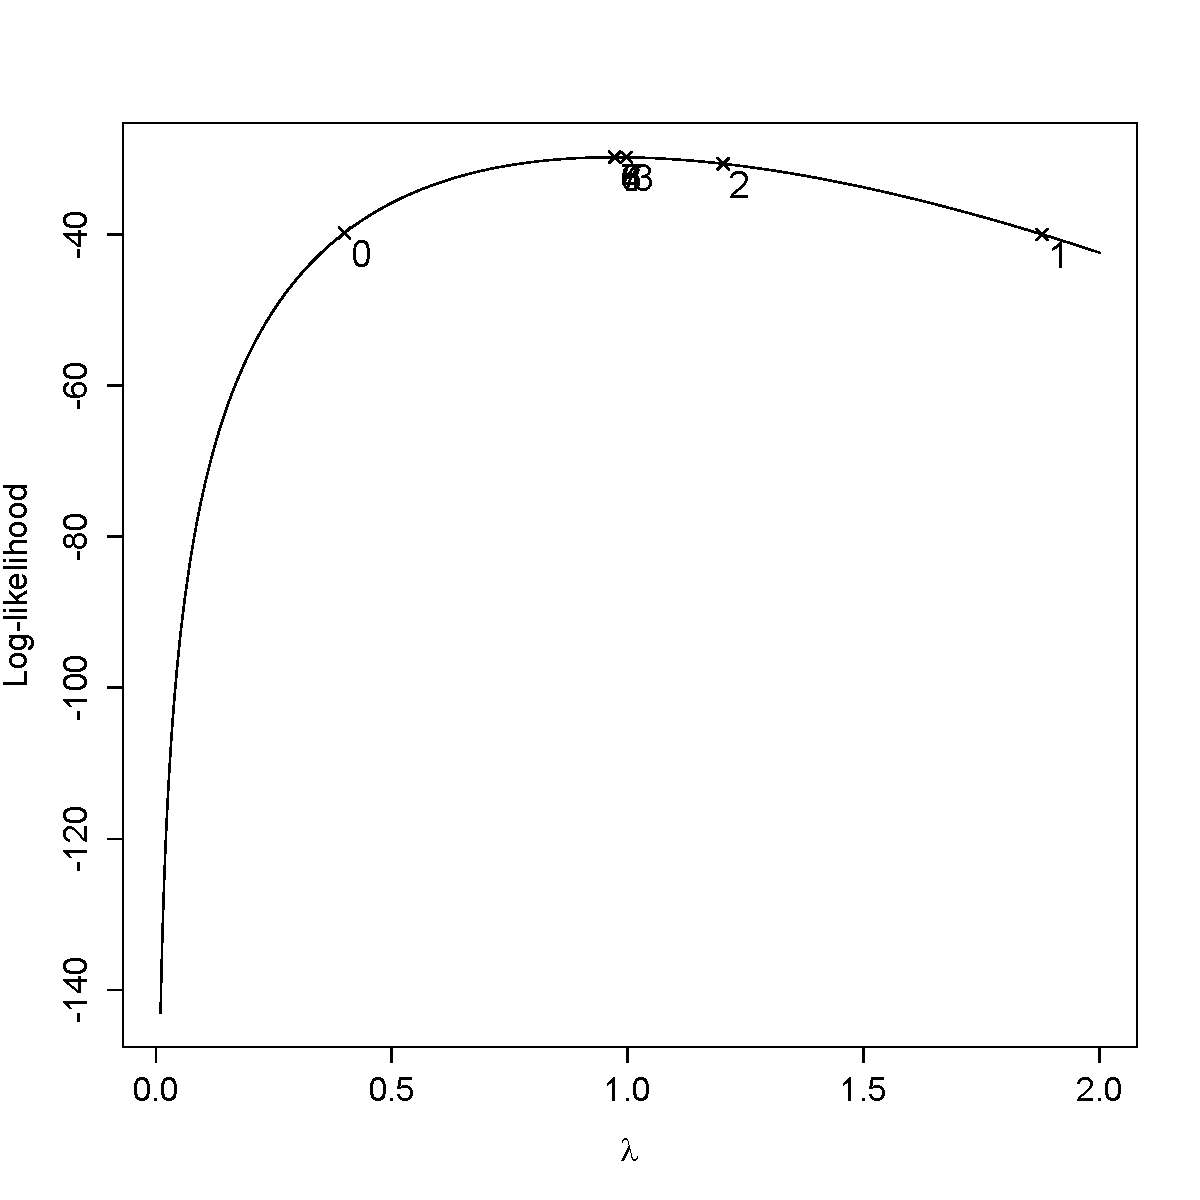
\includegraphics[width=8cm]{NewtonR_meng.pdf}
\caption{Rapid convergence of Newton--Raphson with constraints.}
\label{fig:1}
\end{figure}

 
 \newpage
\section{What if we ignore the constraint?}


\begin{Verbatim}[frame=lines]
ll.expr <- expression(n*(xbar*log(lambda)-lambda-log(1-exp(-lambda))))

dll.expr <- D(ll.expr,"lambda")
ddll.expr <- D(dll.expr,"lambda")

f <- function(lambda) eval(dll.expr) 
df <- function(lambda) eval(ddll.expr) 

# The "data"
n <- 55
xbar <- 1.56363636363636

# Finding the MLE
lambda0 <- 0.4
newtRap(lambda0,10^-6,f,df)
# Seems to work
# What about a more extreme starting value
lambda0 <- 10^-10
newtRap(lambda0,10^-15,f,df)
# Seems to work
# What about a more extreme starting value
lambda0 <- 10^-15
newtRap(lambda0,10^-15,f,df)
\end{Verbatim}





\bibliographystyle{dcu_etal_}
\bibliography{References-cm2011}


\end{document}